\documentclass[UTF8,a4paper,11pt]{ctexart}

\usepackage{geometry}
\geometry{left=2.2cm,right=2.2cm,top=2.4cm,bottom=2.4cm,headheight=14pt,headsep=0.4cm}

\usepackage{graphicx}
\usepackage{booktabs}
\usepackage{array}
\usepackage{tabularx}
\usepackage{enumitem}
\usepackage{xcolor}
\usepackage{fancyhdr}
\usepackage{titlesec}
\usepackage{tcolorbox}
\usepackage{tikz}
\usetikzlibrary{arrows.meta,positioning,fit,calc}

\definecolor{main}{RGB}{38,70,83}
\definecolor{sub}{RGB}{233,236,239}

\pagestyle{fancy}
\fancyhf{}
\lhead{实验3 同步时序部件设计}
\rhead{\thepage}
\renewcommand{\headrulewidth}{0.4pt}

\titleformat{\section}{\Large\bfseries\color{main}}{\thesection}{0.6em}{}
\titleformat{\subsection}{\large\bfseries\color{main}}{\thesubsection}{0.5em}{}

\setlist[itemize]{leftmargin=2em,itemsep=0.3em,topsep=0.3em}
\setlist[enumerate]{leftmargin=2em,itemsep=0.3em,topsep=0.3em}

\newcommand{\blankline}[1]{\vspace{0.25em}\noindent\rule{#1}{0.4pt}\vspace{0.25em}}
\newcommand{\placeholder}[1]{
\begin{tcolorbox}[colback=sub,colframe=main,boxrule=0.6pt,arc=2mm,left=2mm,right=2mm,top=1mm,bottom=1mm]
#1
\end{tcolorbox}
}
\newcommand{\truthtable}[4]{%
\par\medskip
\noindent\begin{tcolorbox}[colback=white,colframe=main,boxrule=0.8pt,arc=2mm,left=1.5mm,right=1.5mm,top=1mm,bottom=1mm]
\centering\bfseries #1\par\smallskip
\renewcommand{\arraystretch}{0.75}
\begin{tabular}{#2}
\toprule
#3\\
\midrule
#4
\bottomrule
\end{tabular}
\end{tcolorbox}
\par\medskip%
}
\newcommand{\figureplaceholder}[2]{
\par\medskip
\noindent\begin{tcolorbox}[colback=white,colframe=main,boxrule=0.8pt,arc=2mm,left=1.5mm,right=1.5mm,top=1mm,bottom=1mm]
\centering\bfseries #1\par\smallskip
\IfFileExists{figures/#2}{%
\includegraphics[width=0.80\linewidth,height=0.88\textheight,keepaspectratio]{figures/\detokenize{#2}}%
}{%
\fbox{\parbox[c][6cm][c]{0.80\linewidth}{\centering 图片请放在 figures/\texttt{\detokenize{#2}}}}
}%
\end{tcolorbox}
\par\medskip
}
\newcommand{\riskimage}[2]{%
\begin{minipage}[t]{0.31\linewidth}
\centering
\includegraphics[height=3.75cm]{figures/\detokenize{#1}}\par
{\small #2}
\end{minipage}%
}

\begin{document}

\begin{center}
{\Huge\bfseries 实验报告}\\[0.8em]
{\LARGE 实验3 同步时序部件设计}\\[1.2em]
\end{center}

\begin{tcolorbox}[colback=white,colframe=main,boxrule=0.8pt,arc=2mm]
\renewcommand{\arraystretch}{1.6}
\begin{tabularx}{\textwidth}{>{\bfseries}p{2.6cm}X >{\bfseries}p{2.6cm}X}
课程名称 & 数字逻辑与计算机组成 & 指导教师 & 吴海军 \\
\end{tabularx}
\end{tcolorbox}

\section{实验目的}
\placeholder{\begin{itemize}
\item 掌握时序逻辑电路设计的基本方法。
\item 掌握计数器和移位寄存器的设计方法和应用。
\item 掌握无符号乘法器、寄存器堆、数字时钟等复杂时序部件的设计方法。
\end{itemize}}

\section{实验环境}
\placeholder{\begin{itemize}
\item 平台：Logisim 2.16
\end{itemize}}

\section{实验内容}

\subsection{计数器实验}

\subsubsection{实验整体方案设计}
\placeholder{\begin{itemize}
\item 顶层模块设计：实验电路较为简单，不需要顶层模块设计图。
\item 输入输出引脚：
\par\medskip
\noindent\begin{tcolorbox}[colback=white,colframe=main,boxrule=0.8pt,arc=2mm,left=1.5mm,right=1.5mm,top=1mm,bottom=1mm]
\renewcommand{\arraystretch}{1.35}
\begin{tabularx}{\textwidth}{>{\bfseries}p{3.2cm}X}
\hline
CLK & 时钟信号 \\
\hline
D0,D1,D2,D3 & 初始输入值 \\
\hline
CLR & 置 1 时清零计数器的值 \\
\hline
ENT,ENP & 使能端，均为 1 时计数器正常计数，至少 1 个为 0 时保持存储之前的计数值 \\
\hline
LD & LD 为 1（且 CLR 为 0）时载入初始输入值 \\
\hline
Q0,Q1,Q2,Q3 & 计数器输出端（输出次态） \\
\hline
RCO & 指示器，Q0,Q1,Q2,Q3 均为 1 时为 1，否则为 0 \\
\hline
\end{tabularx}
\end{tcolorbox}
\end{itemize}}

\subsubsection{实验原理图和电路图}
\figureplaceholder{4位同步二进制计数器原理图}{counter_principle.png}
\figureplaceholder{4位二进制计数器电路图}{counter_circuit.png}

\subsubsection{实验数据仿真测试图}
\figureplaceholder{4位同步二进制计数器仿真测试图}{counter_simulation.png}

\subsubsection{错误现象及分析}
\placeholder{错误现象为电路中发生振荡。错误原因为没有将D触发器设置为沿下降沿触发。修改后运行正常，成功通过了测试。}
\figureplaceholder{4位同步二进制计数器错误现象截图}{counter_error.png}

\subsection{移位寄存器实验}

\subsubsection{实验整体方案设计}
\placeholder{\begin{itemize}
\item 顶层模块设计：实验电路较为简单，不需要顶层模块设计图。
\item 输入输出引脚：
\par\medskip
\noindent\begin{tcolorbox}[colback=white,colframe=main,boxrule=0.8pt,arc=2mm,left=1.5mm,right=1.5mm,top=1mm,bottom=1mm]
\renewcommand{\arraystretch}{1.35}
\begin{tabularx}{\textwidth}{>{\bfseries}p{3.0cm}X}
\hline
CLK & 时钟信号 \\
\hline
CLR\_L & 置为 0 时清零（即低电平有效） \\
\hline
S1,S0 & 控制端，全 0 时保持，全 1 时装载，S1=1、S0=0 时右移，S1=0、S0=1 时左移 \\
\hline
LIN\ RIN & 分别为左移和右移时移入的值 \\
\hline
D3D0 & 初始值 \\
\hline
Q3Q1 & 输出值（次态） \\
\hline
\end{tabularx}
\end{tcolorbox}
\end{itemize}}
    
\subsubsection{实验原理图和电路图}
\figureplaceholder{4位异步移位寄存器原理图}{shiftreg_principle.png}
\figureplaceholder{4位异步移位寄存器电路图}{shiftreg_circuit.png}

\subsubsection{实验数据仿真测试图}
\figureplaceholder{4位异步移位寄存器仿真测试图}{shiftreg_simulation.png}

\subsubsection{错误现象及分析}
\placeholder{实验中没有发生错误。}

\subsection{4 位无符号数乘法器}

\subsubsection{实验整体方案设计}
\placeholder{\begin{itemize}
\item 顶层模块设计：见后图。
\item 输入输出引脚：
\par\medskip
\noindent\begin{tcolorbox}[colback=white,colframe=main,boxrule=0.8pt,arc=2mm,left=1.5mm,right=1.5mm,top=1mm,bottom=1mm]
\renewcommand{\arraystretch}{1.35}
\begin{tabularx}{\textwidth}{>{\bfseries}p{3.0cm}X}
\hline
CLK & 时钟信号 \\
\hline
RST & 清零控制 \\
\hline
X,Y & 两个二进制无符号数 \\
\hline
Z & 乘积输出 \\
\hline
\end{tabularx}
\end{tcolorbox}
\end{itemize}}
\figureplaceholder{4位无符号数乘法器顶层模块设计图}{multiplier_topdesign.png}

\subsubsection{实验原理图和电路图}
 
\figureplaceholder{4位无符号数乘法器组件原理图}{multiplier_principle.png}
\figureplaceholder{4位无符号数乘法器组件电路图}{multiplier_circuit.png}

\subsubsection{实验数据仿真测试图}
\par\medskip
\noindent\begin{tcolorbox}[colback=white,colframe=main,boxrule=0.8pt,arc=2mm,left=1.5mm,right=1.5mm,top=1mm,bottom=1mm]
\centering\bfseries 4位无符号数乘法器仿真测试图\par\smallskip
\begin{minipage}[t]{0.48\linewidth}
\centering
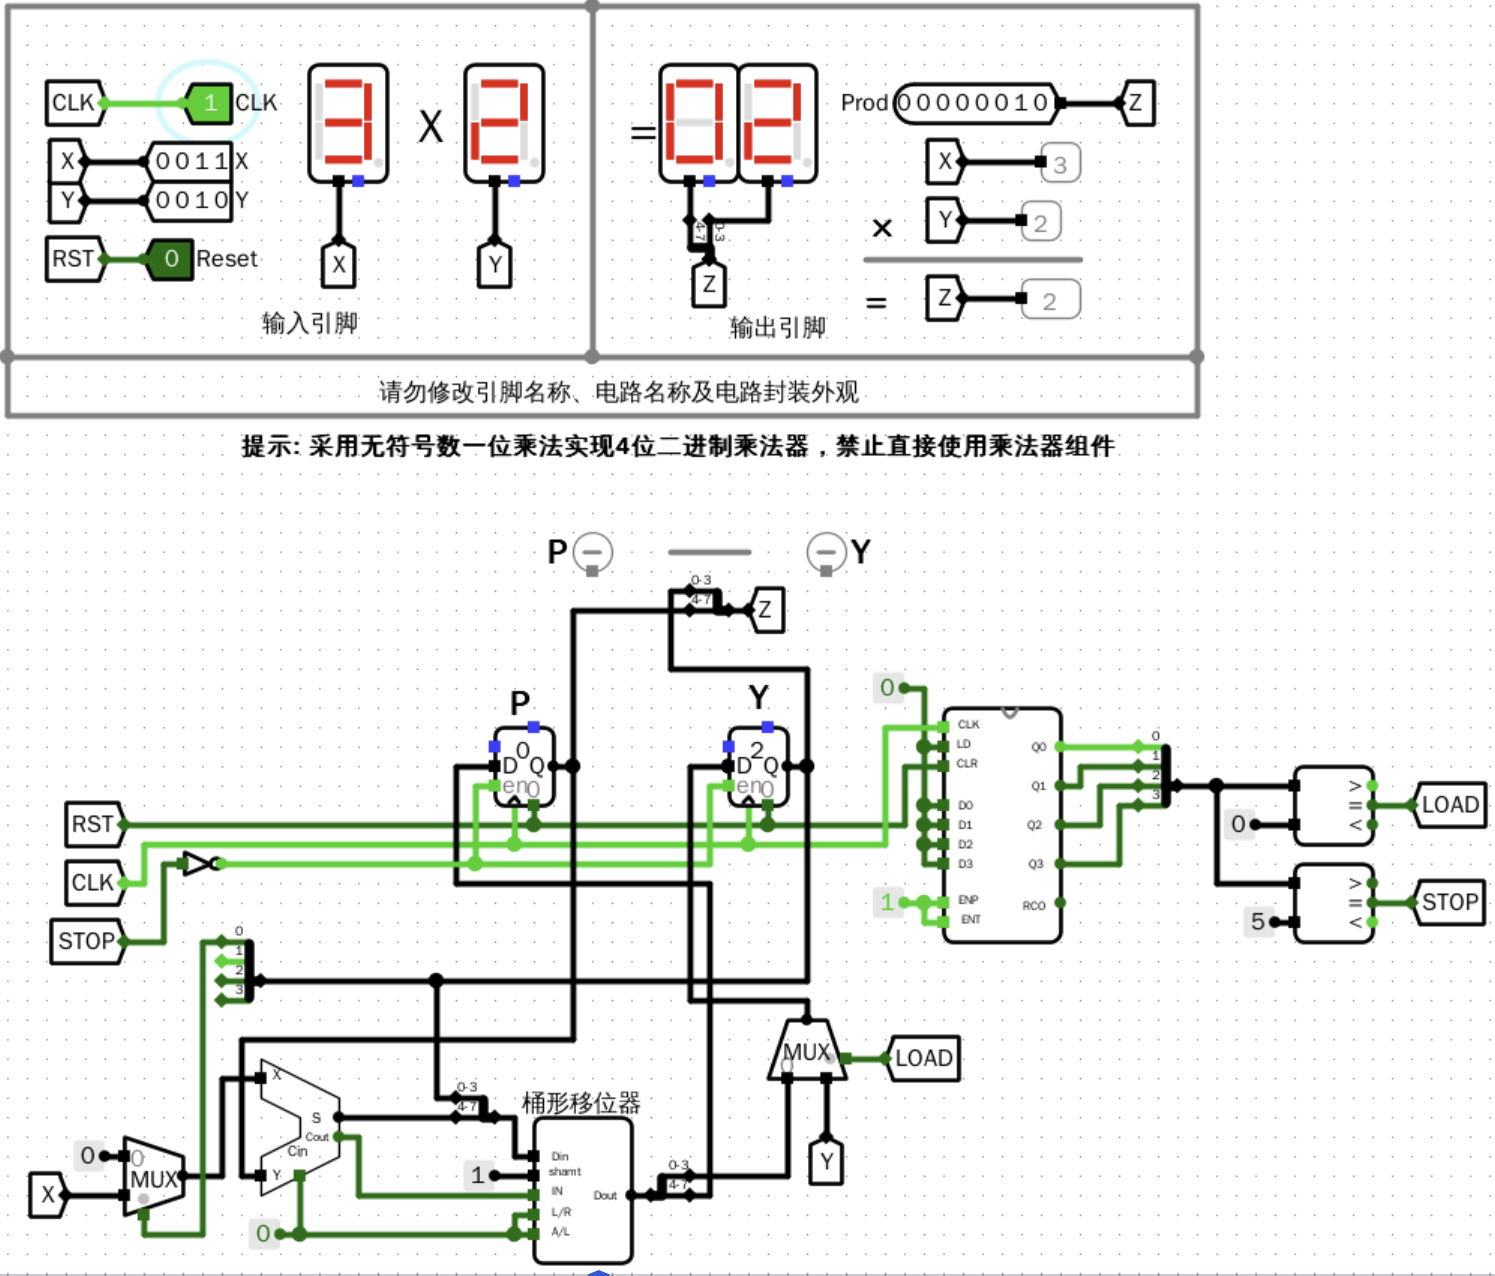
\includegraphics[height=3.25cm]{figures/multiplier_simulation_1.png}\par
{\small 仿真测试图 1}
\end{minipage}\hfill
\begin{minipage}[t]{0.48\linewidth}
\centering
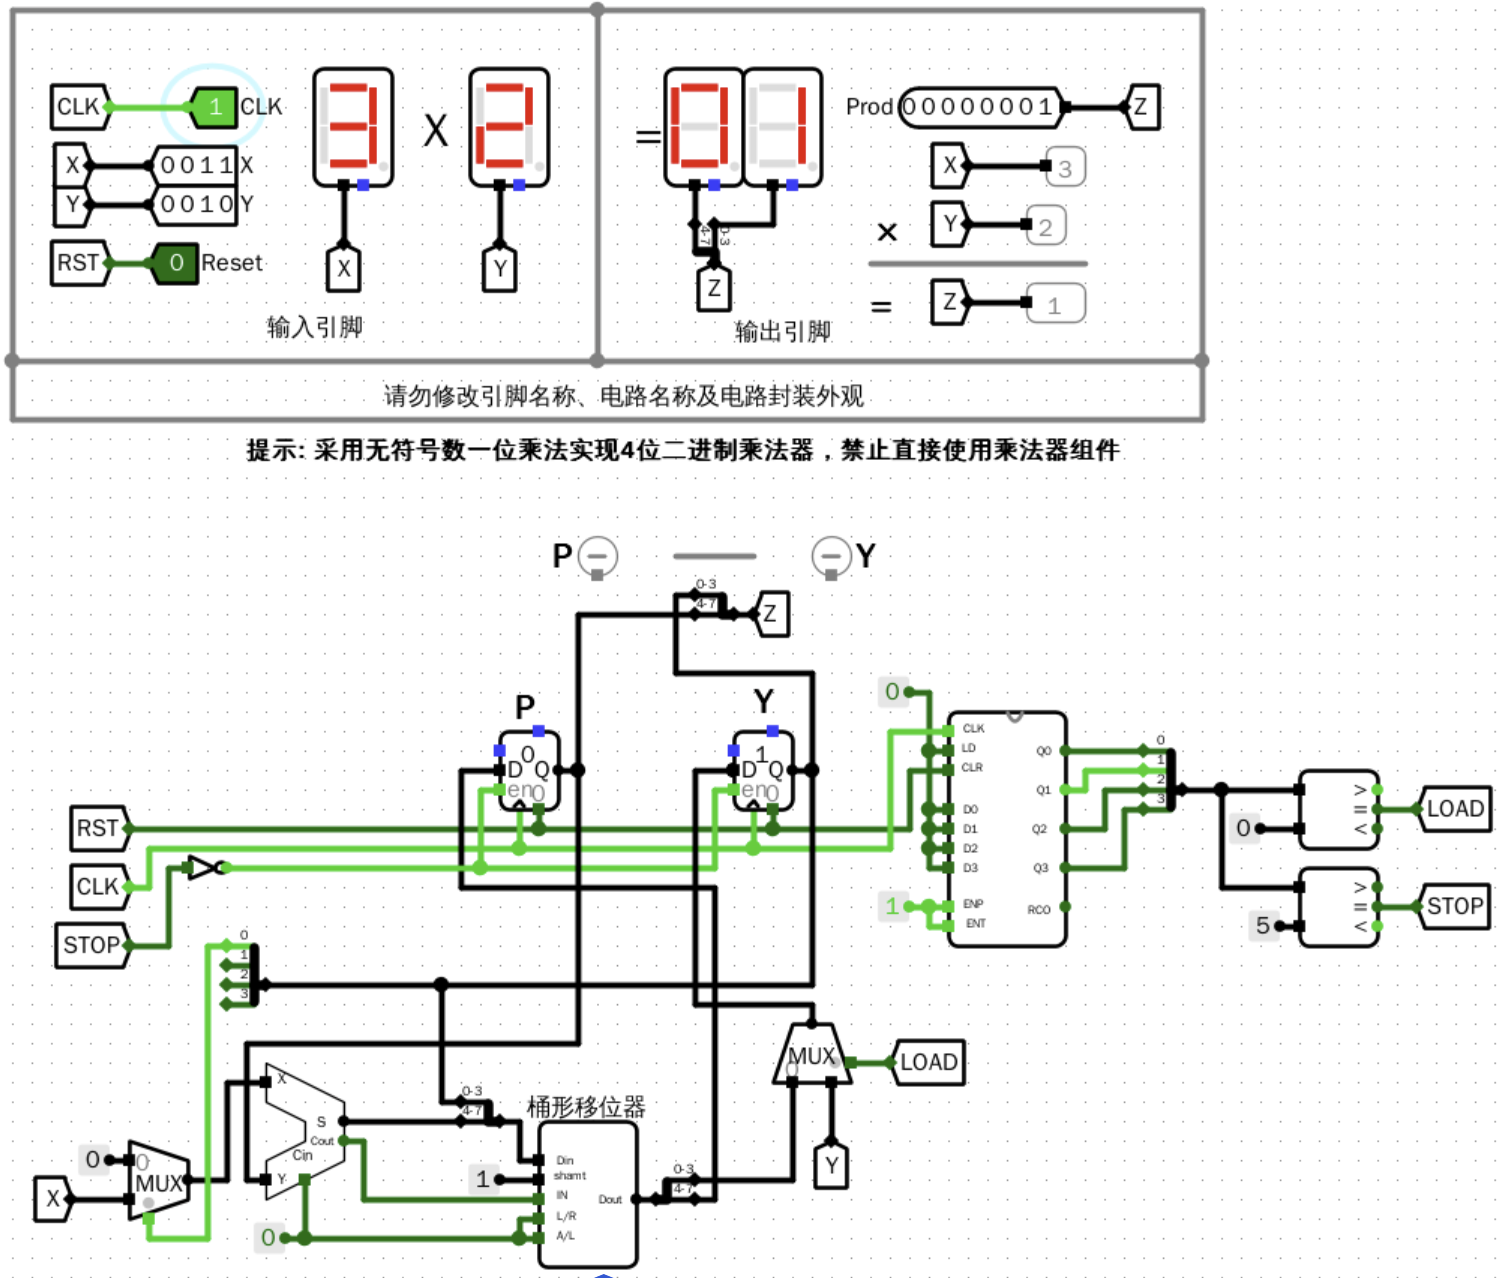
\includegraphics[height=3.25cm]{figures/multiplier_simulation_2.png}\par 
{\small 仿真测试图 2}
\end{minipage}

\vspace{0.8em}

\begin{minipage}[t]{0.48\linewidth}
\centering
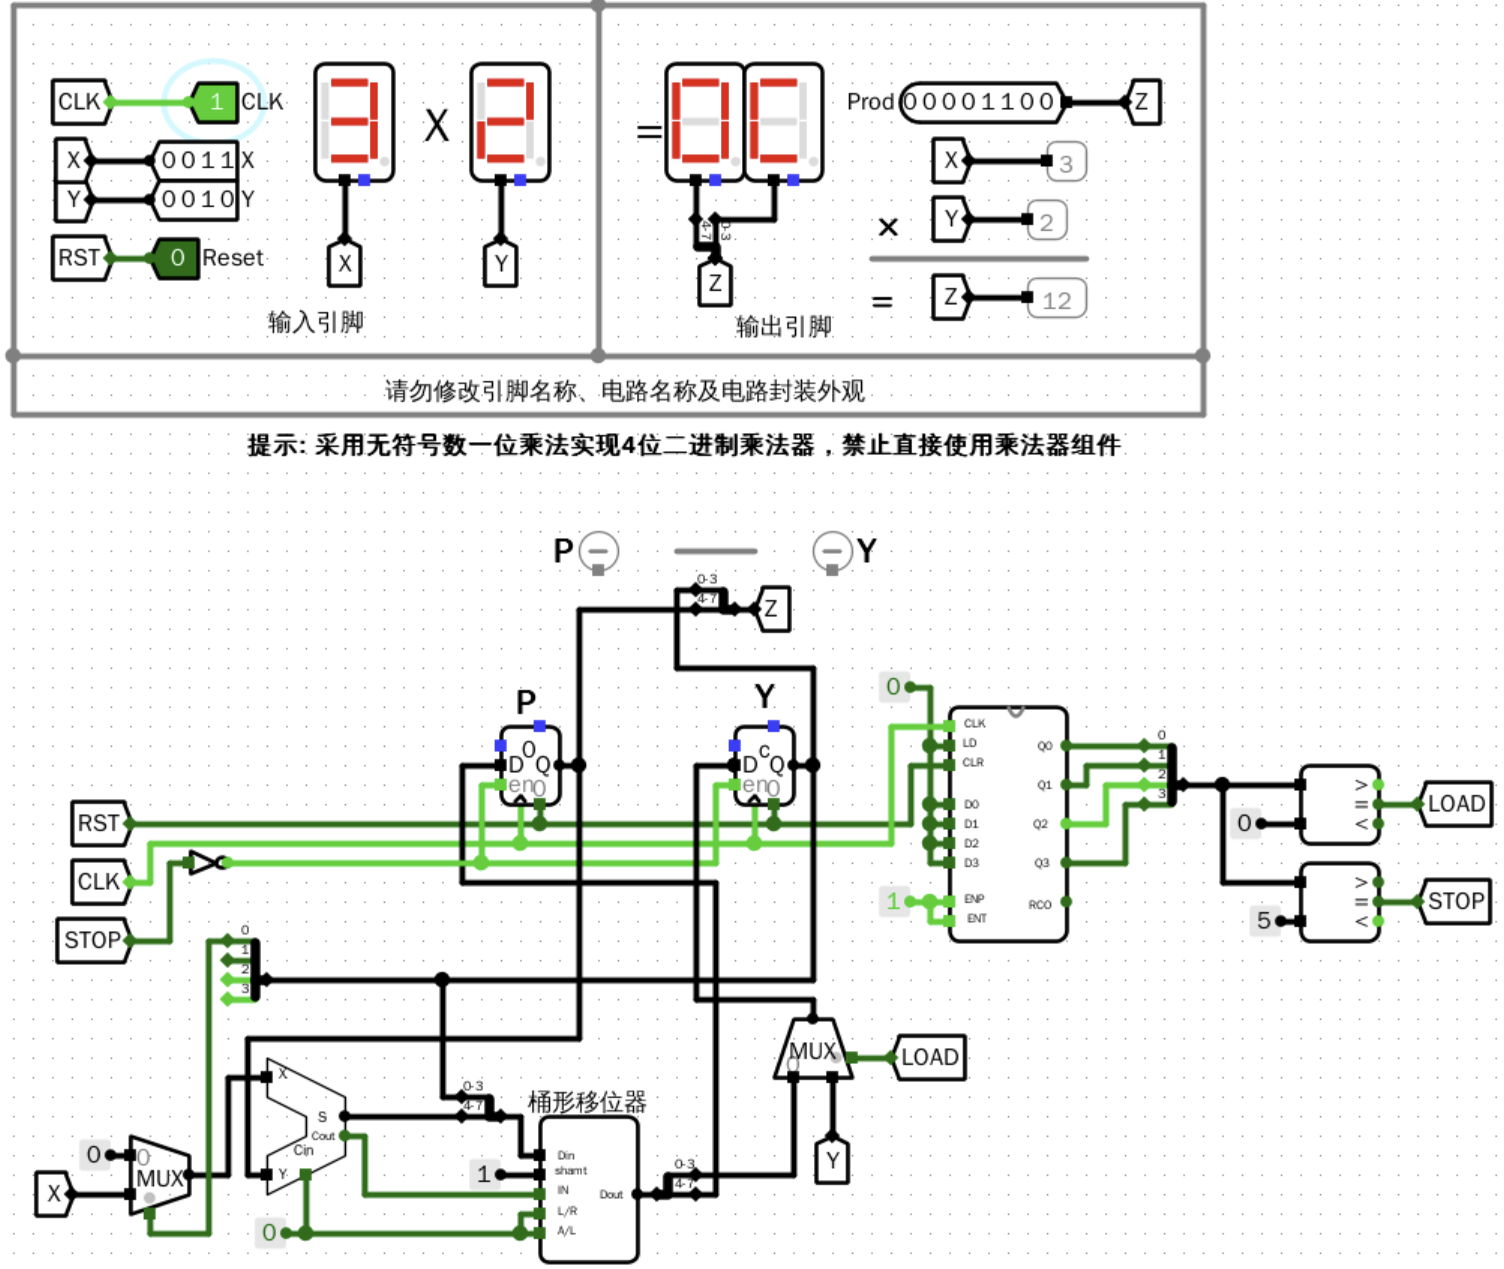
\includegraphics[height=3.25cm]{figures/multiplier_simulation_3.png}\par
{\small 仿真测试图 3}
\end{minipage}\hfill
\begin{minipage}[t]{0.48\linewidth}
\centering
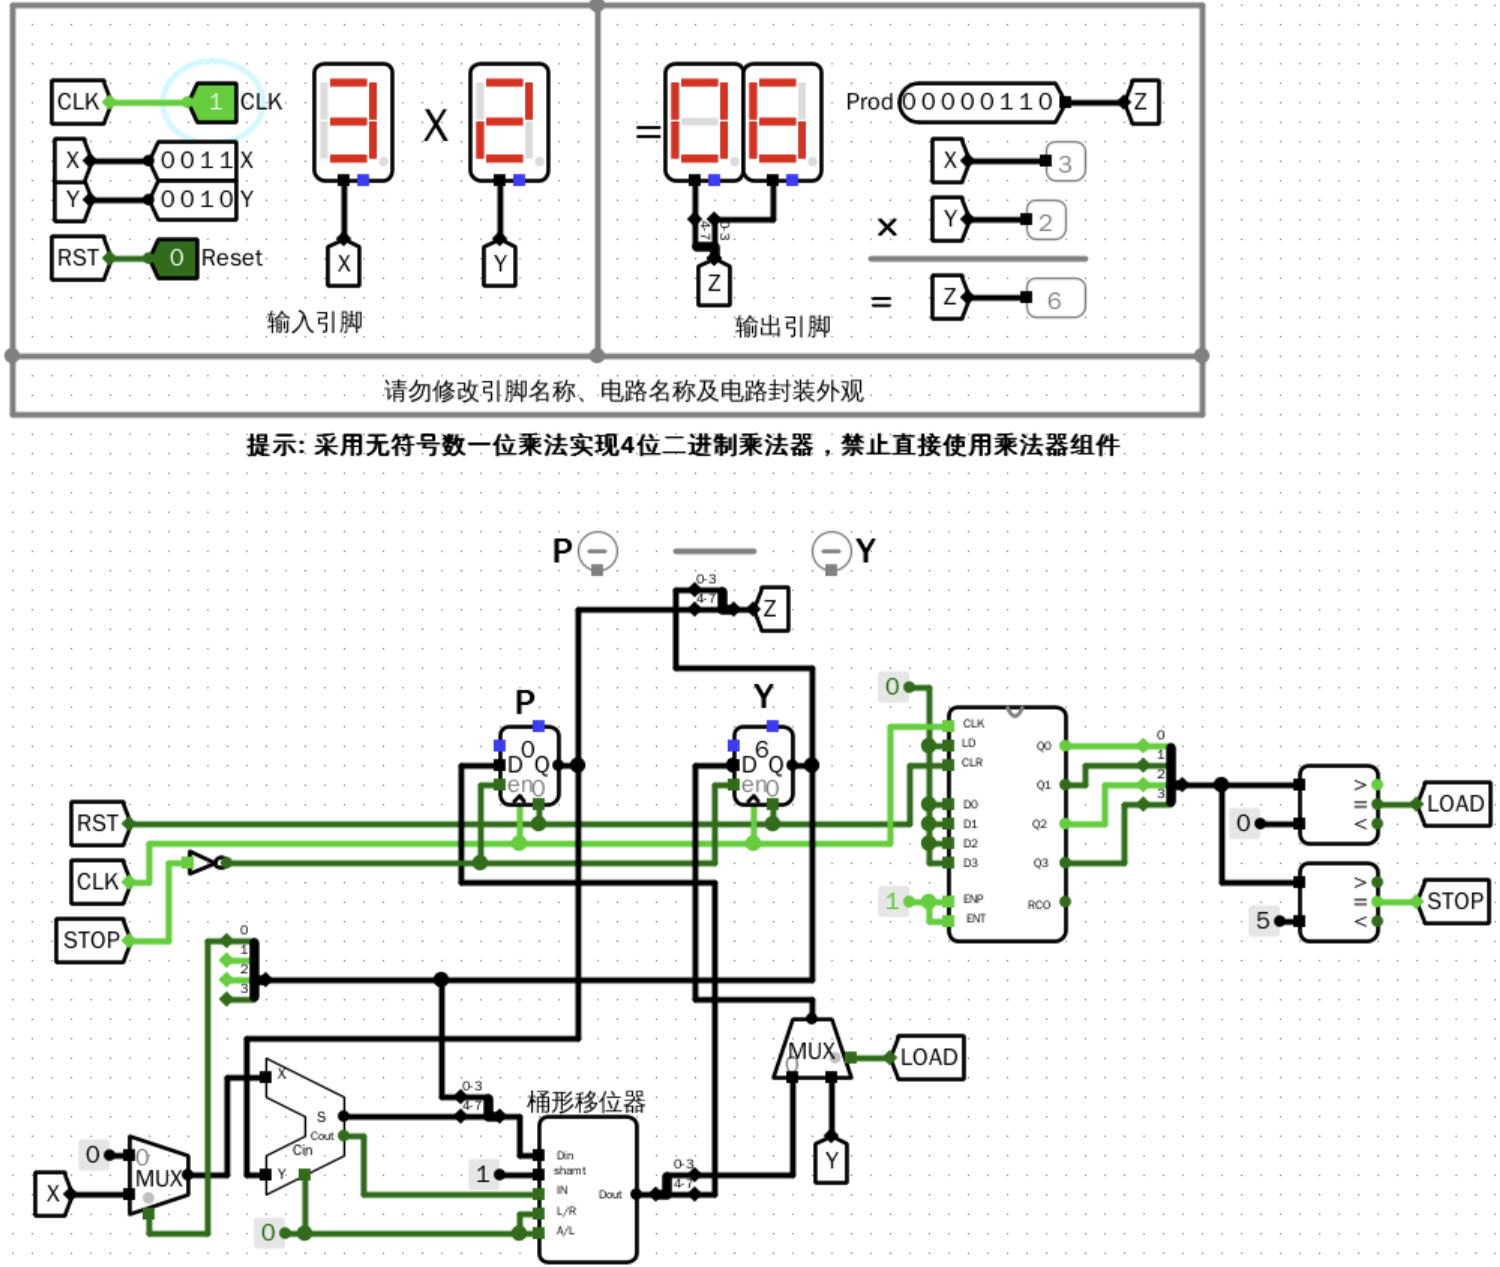
\includegraphics[height=3.25cm]{figures/multiplier_simulation_4.png}\par
{\small 仿真测试图 4}
\end{minipage}
\end{tcolorbox}

\subsubsection{错误现象及分析}
\placeholder{实验中没有发生错误。}

\subsection{寄存器堆实验}

\subsubsection{实验整体方案设计}
\placeholder{\begin{itemize}
\item 顶层模块设计：实验电路较为简单，不需要顶层模块设计图。
\item 输入输出引脚：
\par\medskip
\noindent\begin{tcolorbox}[colback=white,colframe=main,boxrule=0.8pt,arc=2mm,left=1.5mm,right=1.5mm,top=1mm,bottom=1mm]
\renewcommand{\arraystretch}{1.35}
\begin{tabularx}{\textwidth}{>{\bfseries}p{3.0cm}X}
\hline
RW & 控制写入某个寄存器 \\
\hline
WE & 写使能信号 \\
\hline
CLK & 时钟信号 \\
\hline
DIN & 输入数据 \\
\hline
RA\ RB & 控制读取某个寄存器的值 \\
\hline
\end{tabularx}
\end{tcolorbox}
\end{itemize}}

\subsubsection{实验原理图和电路图}
\figureplaceholder{寄存器堆原理图}{regfile_principle.png}
\figureplaceholder{寄存器堆电路图}{regfile_circuit.png}

\subsubsection{实验数据仿真测试图}
\figureplaceholder{寄存器堆仿真测试图}{regfile_simulation.png}

\subsubsection{错误现象及分析}
\placeholder{实验中没有发生错误。}

\subsection{数字时钟实验}

\subsubsection{实验整体方案设计}
\placeholder{\begin{itemize}
\item 顶层模块设计：实验电路较为简单，不需要顶层模块设计图。
\item 输入输出引脚：
\par\medskip
\noindent\begin{tcolorbox}[colback=white,colframe=main,boxrule=0.8pt,arc=2mm,left=1.5mm,right=1.5mm,top=1mm,bottom=1mm]
\renewcommand{\arraystretch}{1.35}
\begin{tabularx}{\textwidth}{>{\bfseries}p{4.0cm}X}
\hline
CLK & 时钟信号 \\
\hline
LD & 控制载入初始时间（高电平有效） \\
\hline
HH\ MM\ SS\ 0(1) & 初始时间（BCD 码） \\
\hline
INErr & 检测初试时间是否有误 \\
\hline
LED & 通过 RGB 三原色实现多种颜色 \\
\hline
\end{tabularx}
\end{tcolorbox}
\end{itemize}}

\subsubsection{实验原理图和电路图}
\figureplaceholder{数字时钟原理图}{clock_principle.png}
\figureplaceholder{BCD码错误检测和三色LED显示信号生成电路图}{clock_errorled_circuit.png}
\figureplaceholder{数字时钟主体电路图}{clock_main_circuit.png}

\subsubsection{实验数据仿真测试图}
\placeholder{在此填写数字时钟的仿真测试说明。}
\figureplaceholder{数字时钟仿真测试图1}{clock_simulation_1.png}
\figureplaceholder{数字时钟仿真测试图2}{clock_simulation_2.png}

\subsubsection{错误现象及分析}
\placeholder{设计的数字时钟在 23:59:59 时无法正确过渡到 00:00:00，显示为 24:00:00。错误原因是没有正确处理小时数的进位条件，组合逻辑设计错误。修改后运行正常，成功通过了测试。}
\figureplaceholder{数字时钟仿真错误截图1}{clock_error_1.png}
\figureplaceholder{数字时钟仿真错误截图2}{clock_error_2.png}

\section{思考题}

\subsection{修改同步计数器电路设计，实现异步清零和异步置数的 4 位计数器，并说明该计数器的应用特性。}
\placeholder{
    使用D触发器的置位和清空功能即可。保存在文件 lab3.6.circ 中。

    应用特性：
    \begin{itemize}
        \item 异步清零：无需等待时钟周期，可以在紧急情况下立即复位计数器。
        \item 异步置数：无需等待时钟周期，可以在紧急情况下立即加载预设值。
    \end{itemize}
}
\figureplaceholder{异步清零和异步置数的 4 位计数器}{async_counter.png}

\subsection{如何仅利用 4 位同步加法计数器在不增加其它逻辑门的情况下，实现模 10 计数器。}
\placeholder{
    将连接 RCO 的五路与门更改为第 2、4 路不反转，再将 RCO 连接到每个 D 触发器的清零端即可。保存在文件 lab3.7.circ 中。
}
\figureplaceholder{模 10 计数器}{mod10_counter.png}

\subsection{利用 4 位移位寄存器设计 8 位二进制伪随机序列电路，写出输出序列值。}
\placeholder{
    用 2 片 SHRG4U 级联，初值设置为 00000001，每个时钟周期寄存器进行一次右移，Q0 被移出作为输出，插入 Q4 $\oplus$ Q3 $\oplus$ Q2 $\oplus$ Q0 为最高位。保存在文件 lab3.8.circ 中。

    生成的随机数序列为：

    1 128 64 32 16 136 196 226 113 56 28 142 71 35 145 72 
    164 210 233 116 58 29 14 7 3 129 192 96 48 152 76 38 
    147 73 36 146 201 100 178 217 236 118 59 157 78 39 19 9 
    4 130 65 160 80 168 212 106 181 218 109 182 91 173 214 107 
    53 154 77 166 211 105 52 26 13 134 195 225 240 248 124 190 
    223 111 183 219 237 246 123 189 94 175 215 235 117 186 93 46 
    23 139 69 34 17 8 132 194 97 176 216 108 54 27 141 198 
    227 241 120 60 158 207 231 115 57 156 206 103 51 25 140 70 
    163 209 104 180 90 45 150 75 37 18 137 68 162 81 40 148 
    74 165 82 169 84 42 149 202 229 114 185 220 238 119 187 221 
    110 55 155 205 230 243 121 188 222 239 247 251 253 126 191 95 
    47 151 203 101 50 153 204 102 179 89 172 86 43 21 138 197 
    98 49 24 12 6 131 193 224 112 184 92 174 87 171 85 170 
    213 234 245 250 125 62 159 79 167 83 41 20 10 133 66 33 
    144 200 228 242 249 252 254 255 127 63 31 15 135 67 161 208 
    232 244 122 61 30 143 199 99 177 88 44 22 11 5 2 (1)

    容易验证循环周期为 255，且每个数值在 1 $\sim$ 255 之间出现一次。
}
\figureplaceholder{8 位二进制伪随机序列电路}{prng_circuit.png}

\subsection{如何实现寄存器堆的写后读功能。}
\placeholder{
    通过 MUX 在写后读时进行特判即可。保存在文件 lab3.9.circ 中。
}
\figureplaceholder{寄存器堆写后读功能电路图}{regfile_writeread_circuit.png}

\end{document}
